% Options for packages loaded elsewhere
% Options for packages loaded elsewhere
\PassOptionsToPackage{unicode}{hyperref}
\PassOptionsToPackage{hyphens}{url}
\PassOptionsToPackage{dvipsnames,svgnames,x11names}{xcolor}
%
\documentclass[
  letterpaper,
  DIV=11,
  numbers=noendperiod]{scrartcl}
\usepackage{xcolor}
\usepackage{amsmath,amssymb}
\setcounter{secnumdepth}{-\maxdimen} % remove section numbering
\usepackage{iftex}
\ifPDFTeX
  \usepackage[T1]{fontenc}
  \usepackage[utf8]{inputenc}
  \usepackage{textcomp} % provide euro and other symbols
\else % if luatex or xetex
  \usepackage{unicode-math} % this also loads fontspec
  \defaultfontfeatures{Scale=MatchLowercase}
  \defaultfontfeatures[\rmfamily]{Ligatures=TeX,Scale=1}
\fi
\usepackage{lmodern}
\ifPDFTeX\else
  % xetex/luatex font selection
\fi
% Use upquote if available, for straight quotes in verbatim environments
\IfFileExists{upquote.sty}{\usepackage{upquote}}{}
\IfFileExists{microtype.sty}{% use microtype if available
  \usepackage[]{microtype}
  \UseMicrotypeSet[protrusion]{basicmath} % disable protrusion for tt fonts
}{}
\makeatletter
\@ifundefined{KOMAClassName}{% if non-KOMA class
  \IfFileExists{parskip.sty}{%
    \usepackage{parskip}
  }{% else
    \setlength{\parindent}{0pt}
    \setlength{\parskip}{6pt plus 2pt minus 1pt}}
}{% if KOMA class
  \KOMAoptions{parskip=half}}
\makeatother
% Make \paragraph and \subparagraph free-standing
\makeatletter
\ifx\paragraph\undefined\else
  \let\oldparagraph\paragraph
  \renewcommand{\paragraph}{
    \@ifstar
      \xxxParagraphStar
      \xxxParagraphNoStar
  }
  \newcommand{\xxxParagraphStar}[1]{\oldparagraph*{#1}\mbox{}}
  \newcommand{\xxxParagraphNoStar}[1]{\oldparagraph{#1}\mbox{}}
\fi
\ifx\subparagraph\undefined\else
  \let\oldsubparagraph\subparagraph
  \renewcommand{\subparagraph}{
    \@ifstar
      \xxxSubParagraphStar
      \xxxSubParagraphNoStar
  }
  \newcommand{\xxxSubParagraphStar}[1]{\oldsubparagraph*{#1}\mbox{}}
  \newcommand{\xxxSubParagraphNoStar}[1]{\oldsubparagraph{#1}\mbox{}}
\fi
\makeatother

\usepackage{color}
\usepackage{fancyvrb}
\newcommand{\VerbBar}{|}
\newcommand{\VERB}{\Verb[commandchars=\\\{\}]}
\DefineVerbatimEnvironment{Highlighting}{Verbatim}{commandchars=\\\{\}}
% Add ',fontsize=\small' for more characters per line
\usepackage{framed}
\definecolor{shadecolor}{RGB}{241,243,245}
\newenvironment{Shaded}{\begin{snugshade}}{\end{snugshade}}
\newcommand{\AlertTok}[1]{\textcolor[rgb]{0.68,0.00,0.00}{#1}}
\newcommand{\AnnotationTok}[1]{\textcolor[rgb]{0.37,0.37,0.37}{#1}}
\newcommand{\AttributeTok}[1]{\textcolor[rgb]{0.40,0.45,0.13}{#1}}
\newcommand{\BaseNTok}[1]{\textcolor[rgb]{0.68,0.00,0.00}{#1}}
\newcommand{\BuiltInTok}[1]{\textcolor[rgb]{0.00,0.23,0.31}{#1}}
\newcommand{\CharTok}[1]{\textcolor[rgb]{0.13,0.47,0.30}{#1}}
\newcommand{\CommentTok}[1]{\textcolor[rgb]{0.37,0.37,0.37}{#1}}
\newcommand{\CommentVarTok}[1]{\textcolor[rgb]{0.37,0.37,0.37}{\textit{#1}}}
\newcommand{\ConstantTok}[1]{\textcolor[rgb]{0.56,0.35,0.01}{#1}}
\newcommand{\ControlFlowTok}[1]{\textcolor[rgb]{0.00,0.23,0.31}{\textbf{#1}}}
\newcommand{\DataTypeTok}[1]{\textcolor[rgb]{0.68,0.00,0.00}{#1}}
\newcommand{\DecValTok}[1]{\textcolor[rgb]{0.68,0.00,0.00}{#1}}
\newcommand{\DocumentationTok}[1]{\textcolor[rgb]{0.37,0.37,0.37}{\textit{#1}}}
\newcommand{\ErrorTok}[1]{\textcolor[rgb]{0.68,0.00,0.00}{#1}}
\newcommand{\ExtensionTok}[1]{\textcolor[rgb]{0.00,0.23,0.31}{#1}}
\newcommand{\FloatTok}[1]{\textcolor[rgb]{0.68,0.00,0.00}{#1}}
\newcommand{\FunctionTok}[1]{\textcolor[rgb]{0.28,0.35,0.67}{#1}}
\newcommand{\ImportTok}[1]{\textcolor[rgb]{0.00,0.46,0.62}{#1}}
\newcommand{\InformationTok}[1]{\textcolor[rgb]{0.37,0.37,0.37}{#1}}
\newcommand{\KeywordTok}[1]{\textcolor[rgb]{0.00,0.23,0.31}{\textbf{#1}}}
\newcommand{\NormalTok}[1]{\textcolor[rgb]{0.00,0.23,0.31}{#1}}
\newcommand{\OperatorTok}[1]{\textcolor[rgb]{0.37,0.37,0.37}{#1}}
\newcommand{\OtherTok}[1]{\textcolor[rgb]{0.00,0.23,0.31}{#1}}
\newcommand{\PreprocessorTok}[1]{\textcolor[rgb]{0.68,0.00,0.00}{#1}}
\newcommand{\RegionMarkerTok}[1]{\textcolor[rgb]{0.00,0.23,0.31}{#1}}
\newcommand{\SpecialCharTok}[1]{\textcolor[rgb]{0.37,0.37,0.37}{#1}}
\newcommand{\SpecialStringTok}[1]{\textcolor[rgb]{0.13,0.47,0.30}{#1}}
\newcommand{\StringTok}[1]{\textcolor[rgb]{0.13,0.47,0.30}{#1}}
\newcommand{\VariableTok}[1]{\textcolor[rgb]{0.07,0.07,0.07}{#1}}
\newcommand{\VerbatimStringTok}[1]{\textcolor[rgb]{0.13,0.47,0.30}{#1}}
\newcommand{\WarningTok}[1]{\textcolor[rgb]{0.37,0.37,0.37}{\textit{#1}}}

\usepackage{longtable,booktabs,array}
\usepackage{calc} % for calculating minipage widths
% Correct order of tables after \paragraph or \subparagraph
\usepackage{etoolbox}
\makeatletter
\patchcmd\longtable{\par}{\if@noskipsec\mbox{}\fi\par}{}{}
\makeatother
% Allow footnotes in longtable head/foot
\IfFileExists{footnotehyper.sty}{\usepackage{footnotehyper}}{\usepackage{footnote}}
\makesavenoteenv{longtable}
\usepackage{graphicx}
\makeatletter
\newsavebox\pandoc@box
\newcommand*\pandocbounded[1]{% scales image to fit in text height/width
  \sbox\pandoc@box{#1}%
  \Gscale@div\@tempa{\textheight}{\dimexpr\ht\pandoc@box+\dp\pandoc@box\relax}%
  \Gscale@div\@tempb{\linewidth}{\wd\pandoc@box}%
  \ifdim\@tempb\p@<\@tempa\p@\let\@tempa\@tempb\fi% select the smaller of both
  \ifdim\@tempa\p@<\p@\scalebox{\@tempa}{\usebox\pandoc@box}%
  \else\usebox{\pandoc@box}%
  \fi%
}
% Set default figure placement to htbp
\def\fps@figure{htbp}
\makeatother

\ifLuaTeX
  \usepackage{luacolor}
  \usepackage[soul]{lua-ul}
\else
  \usepackage{soul}
\fi




\setlength{\emergencystretch}{3em} % prevent overfull lines

\providecommand{\tightlist}{%
  \setlength{\itemsep}{0pt}\setlength{\parskip}{0pt}}



 


\KOMAoption{captions}{tableheading}
\makeatletter
\@ifpackageloaded{caption}{}{\usepackage{caption}}
\AtBeginDocument{%
\ifdefined\contentsname
  \renewcommand*\contentsname{Table of contents}
\else
  \newcommand\contentsname{Table of contents}
\fi
\ifdefined\listfigurename
  \renewcommand*\listfigurename{List of Figures}
\else
  \newcommand\listfigurename{List of Figures}
\fi
\ifdefined\listtablename
  \renewcommand*\listtablename{List of Tables}
\else
  \newcommand\listtablename{List of Tables}
\fi
\ifdefined\figurename
  \renewcommand*\figurename{Figure}
\else
  \newcommand\figurename{Figure}
\fi
\ifdefined\tablename
  \renewcommand*\tablename{Table}
\else
  \newcommand\tablename{Table}
\fi
}
\@ifpackageloaded{float}{}{\usepackage{float}}
\floatstyle{ruled}
\@ifundefined{c@chapter}{\newfloat{codelisting}{h}{lop}}{\newfloat{codelisting}{h}{lop}[chapter]}
\floatname{codelisting}{Listing}
\newcommand*\listoflistings{\listof{codelisting}{List of Listings}}
\makeatother
\makeatletter
\makeatother
\makeatletter
\@ifpackageloaded{caption}{}{\usepackage{caption}}
\@ifpackageloaded{subcaption}{}{\usepackage{subcaption}}
\makeatother
\usepackage{bookmark}
\IfFileExists{xurl.sty}{\usepackage{xurl}}{} % add URL line breaks if available
\urlstyle{same}
\hypersetup{
  pdftitle={Environmental Data Analysis in R - Week 01.01},
  colorlinks=true,
  linkcolor={blue},
  filecolor={Maroon},
  citecolor={Blue},
  urlcolor={Blue},
  pdfcreator={LaTeX via pandoc}}


\title{Environmental Data Analysis in R - Week 01.01}
\author{}
\date{}
\begin{document}
\maketitle


\subsection{GEOG 4/5/7 9073: Environmental Analysis in
R}\label{geog-457-9073-environmental-analysis-in-r}

\subsubsection{Week 01.01: Introduction}\label{week-01.01-introduction}

\subsubsection{Dr.~Bitterman}\label{dr.-bitterman}

\subsection{Today's schedule}\label{todays-schedule}

\begin{itemize}
\tightlist
\item
  Open discussion
\item
  Course welcome
\item
  Introductions
\item
  R basics and practice
\end{itemize}

\subsection{Anything to discuss?
Questions?}\label{anything-to-discuss-questions}

\subsection{My approach to this
course}\label{my-approach-to-this-course}

\begin{itemize}
\tightlist
\item
  Geography matters
\item
  Concepts and independent thinking are important, trivia is not (or at
  least not always)
\item
  It's important to solve problems or complete tasks, but understanding
  HOW you do so is more important
\end{itemize}

\subsection{What this class is}\label{what-this-class-is}

\begin{itemize}
\tightlist
\item
  Collaborative
\item
  Flexible
\item
  \textbf{\emph{Student-led}}
\end{itemize}

\paragraph{What else it is}\label{what-else-it-is}

\begin{itemize}
\tightlist
\item
  A bit mis-named
\item
  My second time teaching it here at KSU - so we have space to
  experiment a bit
\end{itemize}

\subsection{Class introductions}\label{class-introductions}

Pair up -- and don't leave anyone behind

\textbf{Share:}

\begin{itemize}
\item
  Name
\item
  Where you're from
\item
  Major/program, year
\item
  Why are you taking this course?
\item
  Why are you in your major? Why KSU?
\item
  Previous experience: GIS, programming, R?
\item
  Imagine it's May 2026 -- what would make you feel like you were
  successful in this course. SAVE THIS SOMEWHERE!!!
\end{itemize}

\subsection{My introduction}\label{my-introduction}

\begin{itemize}
\tightlist
\item
  Dr.~Patrick Bitterman
\item
  Independence, IA -\textgreater{} UIowa -\textgreater{} UVM
  -\textgreater{} UNL -\textgreater{} KSU
\item
  Assistant Professor in Geography Department, 2nd/7th year
\item
  Goals: teach a successful course, build my research program
\item
  GIS experience? Programming experience? Extensive, but I don't use
  ArcGIS much\ldots{}
\item
  Success in this course:

  \begin{itemize}
  \tightlist
  \item
    students reach \emph{their} learning objectives
  \item
    students are able to use R to make their work faster and more
    consistent
  \item
    students improve methods related to their other research or career
    interests
  \item
    students develop an appreciation for programmatic spatial analysis
  \end{itemize}
\end{itemize}

\subsection{Time to share}\label{time-to-share}

\begin{itemize}
\tightlist
\item
  Present your partner to the class
\item
  Who wants to go first?
\end{itemize}

\emph{Share:}

\begin{itemize}
\item
  Name
\item
  Where you're from
\item
  Major/program, year
\item
  Why are you taking this course?
\item
  Why are you in your major? Why KSU?
\item
  Previous experience: GIS, programming, R?
\item
  What would make you feel successful?
\end{itemize}

\subsection{Course basics}\label{course-basics}

\subsection{Instructor (me)}\label{instructor-me}

\begin{itemize}
\item
  Dr.~Patrick Bitterman
\item
  Geography Department
\item
  Office: 436 McGilvrey Hall
\item
  Office hours: MW 9-11am, or by appointment
\item
  Email: pbitterm@kent.edu
\end{itemize}

\subsection{Materials}\label{materials}

\begin{itemize}
\item
  Brunsdon, C., Comber, L. 2025. An Introduction to R for Spatial
  Analysis and Mapping (Spatial Analytics and GIS). 3rd Edition. SAGE.
  \href{https://collegepublishing.sagepub.com/products/an-introduction-to-r-for-spatial-analysis-and-mapping-3-288946}{Link}
\item
  Optional: Wickham, H. 2017. R for Data Science: Import, Tidy,
  Transform, Visualize, and Model Data. O'Reilly Media. (if you are
  unfamiliar with R or other programming language)
  (\url{https://r4ds.had.co.nz/index.html)}
\end{itemize}

\subsection{Learning objectives}\label{learning-objectives}

By the end of the term, students will be able to successfully:

\begin{itemize}
\tightlist
\item
  Demonstrate a familiarity with the R programming language in the
  context of geospatial analysis
\item
  Write self-contained functions to automate geospatial tasks
\item
  Analyze model workflows and describe computer code and algorithms in
  plain language
\item
  Create small-scale programs that interface with web-based tools
\item
  Practice good programming practices
\item
  Plan, develop, and execute a programmatic analysis of a dataset
\end{itemize}

\subsection{Course policies}\label{course-policies}

\begin{itemize}
\item
  Assignment submission:

  \begin{itemize}
  \item
    All assignments due on their due date
  \item
    All assignments will be posted on Canvas, but turned in via GitHub
    (we'll talk more)
  \item
    Late items will be accepted, but will be penalized 20\% of the
    potential points for each day they are late
  \end{itemize}
\item
  All changes to the syllabus will be communicated via Canvas
  announcement
\item
  Students are expected to attend all class meetings, but attendance is
  not graded. \textbf{Participation is graded, though}
\end{itemize}

\subsection{Collaboration}\label{collaboration}

\begin{itemize}
\tightlist
\item
  Feel free to discuss labs, etc. with your classmates
\item
  However\ldots{}

  \begin{itemize}
  \tightlist
  \item
    All lab reports, papers, and other work should be your own,
    individual thoughts
  \item
    Students who do not follow these policies will be reported to the
    College for academic dishonesty
  \end{itemize}
\end{itemize}

\subsection{Other tips}\label{other-tips}

\begin{itemize}
\tightlist
\item
  Read relevant materials before class
\item
  Attend class -- understanding theory and concepts will help you with
  practical applications
\item
  If there are topics, news stories, blog posts, tweets, etc. that you
  find interesting or want to know more about, let me know
\item
  Before you start coding, think through the process and sketch out the
  workflow. This is called \emph{pseudocode}
\item
  Labs build on each other, so don't get behind
\item
  Take advantage of office hours
\item
  Do not leave assignments until the last minute
\item
  Have fun!
\end{itemize}

\subsection{Assessment}\label{assessment}

\paragraph{Lab assignments}\label{lab-assignments}

\begin{itemize}
\tightlist
\item
  6 labs, 2-3 weeks to complete each one
\end{itemize}

\paragraph{Final project}\label{final-project}

\begin{itemize}
\tightlist
\item
  Proposal
\item
  Update presentation (in-class)
\item
  Final presentation (in-class)
\item
  Final report
\end{itemize}

\paragraph{Participation}\label{participation}

\paragraph{Graduate students}\label{graduate-students}

For graduate students, the requirements of the final project will be
expanded to include:

\begin{enumerate}
\def\labelenumi{\arabic{enumi})}
\tightlist
\item
  an additional 3-4 pages in your report
\item
  code documentation
\item
  an additional 5 minutes in your final presentation to the class.
\item
  required to produce a cover page for your GitHub page/portfolio
\end{enumerate}

\subsection{Course format}\label{course-format}

\begin{itemize}
\tightlist
\item
  Project-based
\item
  Student-led

  \begin{itemize}
  \tightlist
  \item
    I am not going to recap the readings (much)
  \item
    You are expected to be ready to participate in discussion
  \item
    We will spend most of our time doing, not lecturing
  \end{itemize}
\item
  \textbf{Tuesdays}: discussion, examples, and activities
\item
  \textbf{Thursdays}: wildcard day (coding challenges, group work,
  seminar)
\end{itemize}

\subsection{Course inspiration and source
material}\label{course-inspiration-and-source-material}

\begin{itemize}
\tightlist
\item
  My own experience
\item
  Your textbook
\item
  Lovelace, R. \emph{Geocomputation with R}
  \url{https://geocompr.robinlovelace.net/index.html}
\end{itemize}

\subsection{University policies}\label{university-policies}

\begin{itemize}
\tightlist
\item
  Learning accommodations

  \begin{itemize}
  \tightlist
  \item
    Contact Student Support Services
  \item
    Let me know
  \end{itemize}
\item
  Academic integrity

  \begin{itemize}
  \tightlist
  \item
    Don't cheat
  \item
    Don't plagiarize
  \end{itemize}
\item
  Health and safety

  \begin{itemize}
  \tightlist
  \item
    Student support services
    (\url{https://www.kent.edu/studentsupportservices)}
  \end{itemize}
\end{itemize}

\subsection{The Generative AI Elephant in the
Room}\label{the-generative-ai-elephant-in-the-room}

\begin{itemize}
\item
  Yes, ChatGPT, Claude, Copilot, etc. can write code\ldots{}
\item
  \ldots and most of the time, it's even correct
\end{itemize}

\section{For example}\label{for-example}

\pandocbounded{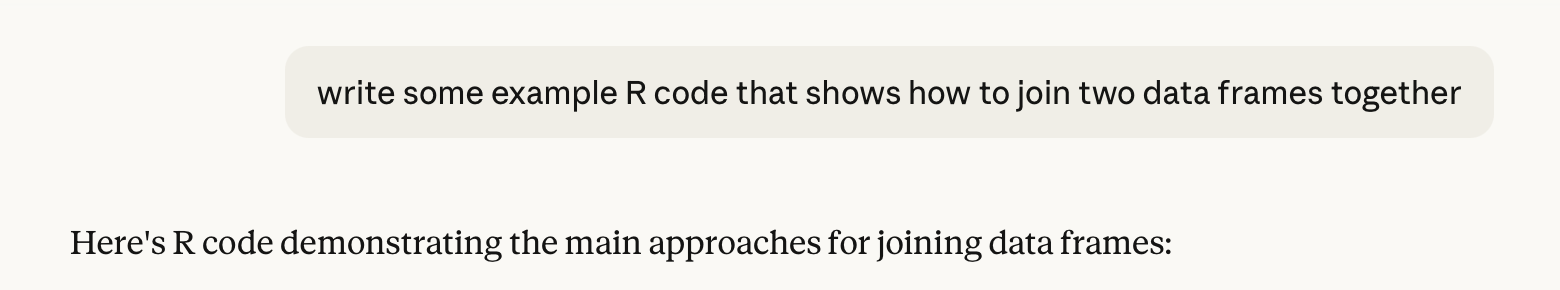
\includegraphics[keepaspectratio]{images/claude.png}}

\begin{Shaded}
\begin{Highlighting}[]
\FunctionTok{library}\NormalTok{(tidyverse)}
\end{Highlighting}
\end{Shaded}

\begin{verbatim}
-- Attaching core tidyverse packages ------------------------ tidyverse 2.0.0 --
v dplyr     1.1.4     v readr     2.1.5
v forcats   1.0.0     v stringr   1.5.1
v ggplot2   3.5.1     v tibble    3.2.1
v lubridate 1.9.3     v tidyr     1.3.1
v purrr     1.0.2     
-- Conflicts ------------------------------------------ tidyverse_conflicts() --
x dplyr::filter() masks stats::filter()
x dplyr::lag()    masks stats::lag()
i Use the conflicted package (<http://conflicted.r-lib.org/>) to force all conflicts to become errors
\end{verbatim}

\begin{Shaded}
\begin{Highlighting}[]
\CommentTok{\# Create example data frames}
\NormalTok{df1 }\OtherTok{\textless{}{-}} \FunctionTok{data.frame}\NormalTok{(}
  \AttributeTok{studentId =} \FunctionTok{c}\NormalTok{(}\DecValTok{1}\NormalTok{, }\DecValTok{2}\NormalTok{, }\DecValTok{3}\NormalTok{, }\DecValTok{4}\NormalTok{),}
  \AttributeTok{name =} \FunctionTok{c}\NormalTok{(}\StringTok{"Alice"}\NormalTok{, }\StringTok{"Bob"}\NormalTok{, }\StringTok{"Carol"}\NormalTok{, }\StringTok{"David"}\NormalTok{),}
  \AttributeTok{score =} \FunctionTok{c}\NormalTok{(}\DecValTok{85}\NormalTok{, }\DecValTok{92}\NormalTok{, }\DecValTok{78}\NormalTok{, }\DecValTok{88}\NormalTok{)}
\NormalTok{)}

\NormalTok{df2 }\OtherTok{\textless{}{-}} \FunctionTok{data.frame}\NormalTok{(}
  \AttributeTok{studentId =} \FunctionTok{c}\NormalTok{(}\DecValTok{2}\NormalTok{, }\DecValTok{3}\NormalTok{, }\DecValTok{4}\NormalTok{, }\DecValTok{5}\NormalTok{),}
  \AttributeTok{department =} \FunctionTok{c}\NormalTok{(}\StringTok{"Biology"}\NormalTok{, }\StringTok{"Chemistry"}\NormalTok{, }\StringTok{"Physics"}\NormalTok{, }\StringTok{"Math"}\NormalTok{),}
  \AttributeTok{year =} \FunctionTok{c}\NormalTok{(}\DecValTok{2}\NormalTok{, }\DecValTok{3}\NormalTok{, }\DecValTok{1}\NormalTok{, }\DecValTok{4}\NormalTok{)}
\NormalTok{)}

\FunctionTok{inner\_join}\NormalTok{(df1, df2, }\AttributeTok{by =} \StringTok{"studentId"}\NormalTok{)}
\end{Highlighting}
\end{Shaded}

\begin{verbatim}
  studentId  name score department year
1         2   Bob    92    Biology    2
2         3 Carol    78  Chemistry    3
3         4 David    88    Physics    1
\end{verbatim}

\subsection{The AI ``discussion''}\label{the-ai-discussion}

In your opinion AND in the context of this class\ldots{}

\begin{itemize}
\item
  What are some arguments FOR using GAI for writing code?
\item
  What are some arguments AGAINST using GAI for writing code?
\item
  What is a reasonable use policy?
\end{itemize}

\subsection{Anything else?}\label{anything-else}

\begin{itemize}
\tightlist
\item
  Questions?
\end{itemize}

\paragraph{Let's look at the Canvas and GitHub
sites}\label{lets-look-at-the-canvas-and-github-sites}

\subsection{Let's talk writing code}\label{lets-talk-writing-code}

\subsection{SA and Programming in R}\label{sa-and-programming-in-r}

\begin{itemize}
\tightlist
\item
  Experience? In what setting?
\item
  Experience with a version control system (e.g., git)?
\item
  What about experience with spatial analysis, GIS?
\end{itemize}

\subsection{Let's make sure we're setup and familiar with R +
RStudio}\label{lets-make-sure-were-setup-and-familiar-with-r-rstudio}

\begin{enumerate}
\def\labelenumi{\arabic{enumi}.}
\item
  Login to your computer if you haven't (you may also use your own)
\item
  Launch RStudio
\item
  Wait
\end{enumerate}

\subsection{R and RStudio: Understanding the
Relationship}\label{r-and-rstudio-understanding-the-relationship}

R and RStudio are c\ul{\textbf{omplementary but distinct tools}} that
work together for data analysis:

\subsubsection{\texorpdfstring{\textbf{R}}{R}}\label{r}

\begin{itemize}
\item
  underlying statistical programming language and computational engine
\item
  performs all calculations, executes code, manages data structures, and
  produces outputs
\item
  can run independently from the command line or terminal
\end{itemize}

\subsubsection{\texorpdfstring{\textbf{RStudio}}{RStudio}}\label{rstudio}

\begin{itemize}
\item
  is an Integrated Development Environment (IDE)
\item
  sends your code to R for execution and displays the results in an
  organized workspace
\item
  means you could use R with different interfaces (VSCode, Jupyter,
  command line), but\ldots{}
\item
  RStudio is purpose-built for R workflows and offers features
  specifically designed for statistical analysis and data science tasks
\end{itemize}

\subsection{The RStudio Interface}\label{the-rstudio-interface}

When you first launch RStudio, you'll see a workspace divided into four
main panes (which you can customize):

\subsubsection{1. Source Pane (Top Left)}\label{source-pane-top-left}

This is your code editor where you write and save R scripts (.R files)
or Quarto/R Markdown documents (.qmd/.Rmd files).

\begin{itemize}
\tightlist
\item
  Write multi-line code that you can save and reuse
\item
  Execute single lines with \texttt{Ctrl+Enter} (Windows/Linux) or
  \texttt{Cmd+Enter} (Mac)
\item
  Execute selected code chunks
\item
  Syntax highlighting helps identify functions, variables, and errors
\item
  Line numbers assist with debugging
\end{itemize}

\ul{\textbf{\emph{Always (mostly) work in scripts rather than only in
the Console---this ensures reproducibility}}}

\begin{center}\rule{0.5\linewidth}{0.5pt}\end{center}

\subsubsection{2. Console Pane (Bottom
Left)}\label{console-pane-bottom-left}

This is where R actually runs and displays output.

\begin{itemize}
\tightlist
\item
  Code executed from the Source pane appears here
\item
  You can type code directly for quick tests or calculations
\item
  Results, messages, warnings, and errors display here
\item
  The \texttt{\textgreater{}} prompt indicates R is ready for input
\item
  The \texttt{+} prompt means R is waiting for you to complete a command
\end{itemize}

\begin{center}\rule{0.5\linewidth}{0.5pt}\end{center}

\subsubsection{3. Environment/History Pane (Top
Right)}\label{environmenthistory-pane-top-right}

\textbf{Environment tab:}

\begin{itemize}
\item
  Shows all objects currently loaded in your R session (e.g., data
  frames, vectors, functions)
\item
  Click on data frames to view them in a spreadsheet-like format
\item
  Displays object types and dimensions
\item
  The broom icon clears your workspace (be careful!)
\end{itemize}

\textbf{History tab:}

\begin{itemize}
\item
  Records all commands you've executed
\item
  Useful for recovering code you ran but didn't save
\end{itemize}

\begin{center}\rule{0.5\linewidth}{0.5pt}\end{center}

\subsubsection{4. Files/Plots/Packages/Help Pane (Bottom
Right)}\label{filesplotspackageshelp-pane-bottom-right}

multi-purpose pane with tabs:

\begin{itemize}
\item
  \textbf{Files}
\item
  \textbf{Plots}
\item
  \textbf{Packages}
\item
  \textbf{Help}
\item
  \textbf{Viewer}
\end{itemize}

\subsection{Let's try it out}\label{lets-try-it-out}

Practice using RStudio by:

\begin{enumerate}
\def\labelenumi{\arabic{enumi}.}
\tightlist
\item
  Creating a new R Script (File \textgreater{} New File \textgreater{} R
  Script)
\item
  Writing simple code (e.g., \texttt{x\ \textless{}-\ 1:10})
\item
  Executing it and observing results in the Console
\item
  Viewing created objects in the Environment pane
\item
  Creating a simple plot and viewing it in the Plots pane
\end{enumerate}

\begin{Shaded}
\begin{Highlighting}[]
\NormalTok{x }\OtherTok{\textless{}{-}} \DecValTok{1}\SpecialCharTok{:}\DecValTok{10}
\NormalTok{y }\OtherTok{\textless{}{-}} \FunctionTok{rnorm}\NormalTok{(}\DecValTok{100}\NormalTok{, }\AttributeTok{mean =} \DecValTok{0}\NormalTok{, }\AttributeTok{sd =} \DecValTok{2}\NormalTok{)}
\NormalTok{x}
\end{Highlighting}
\end{Shaded}

\begin{verbatim}
 [1]  1  2  3  4  5  6  7  8  9 10
\end{verbatim}

\begin{Shaded}
\begin{Highlighting}[]
\NormalTok{x }\SpecialCharTok{*} \DecValTok{2}
\end{Highlighting}
\end{Shaded}

\begin{verbatim}
 [1]  2  4  6  8 10 12 14 16 18 20
\end{verbatim}

\begin{Shaded}
\begin{Highlighting}[]
\FunctionTok{hist}\NormalTok{(y)}
\end{Highlighting}
\end{Shaded}

\pandocbounded{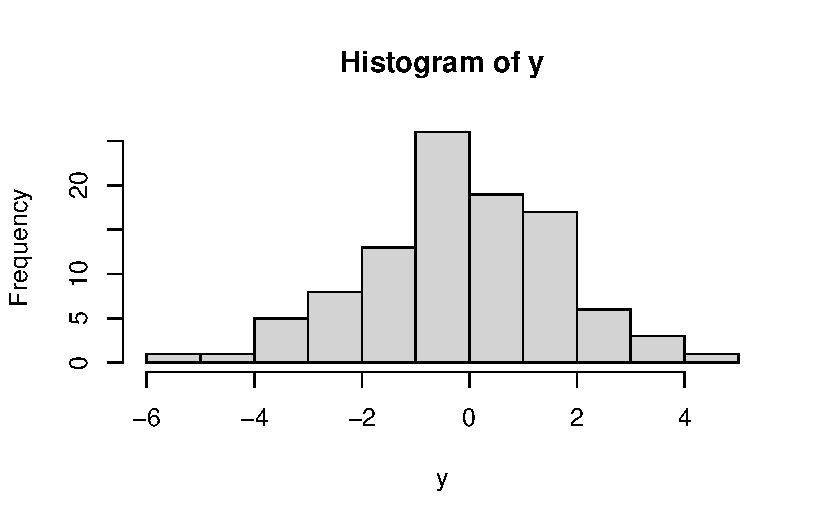
\includegraphics[keepaspectratio]{week01_01_files/figure-pdf/unnamed-chunk-2-1.pdf}}

\begin{center}\rule{0.5\linewidth}{0.5pt}\end{center}

\begin{Shaded}
\begin{Highlighting}[]
\NormalTok{x }\OtherTok{\textless{}{-}} \DecValTok{1}\SpecialCharTok{:}\DecValTok{100}
\NormalTok{y }\OtherTok{\textless{}{-}} \FunctionTok{rnorm}\NormalTok{(}\DecValTok{100}\NormalTok{, }\AttributeTok{mean =} \DecValTok{0}\NormalTok{, }\AttributeTok{sd =} \DecValTok{2}\NormalTok{)}
\FunctionTok{plot}\NormalTok{(x, y)}
\end{Highlighting}
\end{Shaded}

\pandocbounded{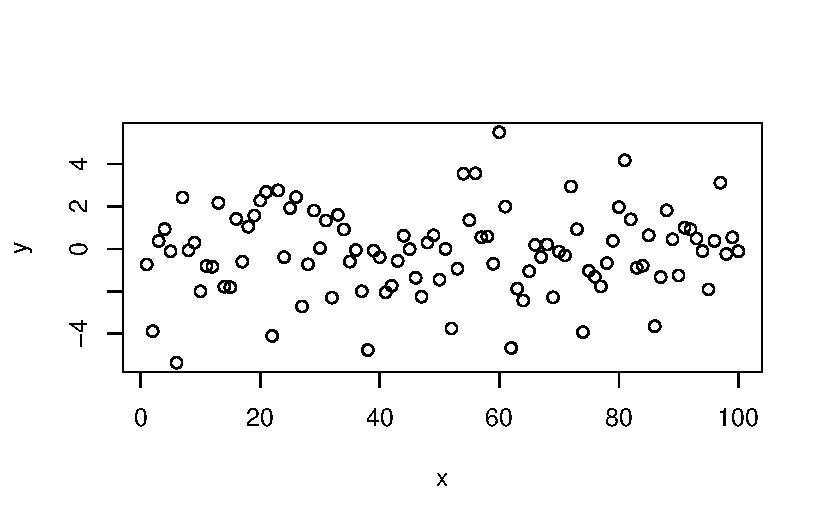
\includegraphics[keepaspectratio]{week01_01_files/figure-pdf/unnamed-chunk-3-1.pdf}}

\subsection{Review and next class}\label{review-and-next-class}

\begin{itemize}
\tightlist
\item
  Any questions on course policies?
\item
  On anything else?
\end{itemize}

\subsubsection{\texorpdfstring{\textbf{This week's
readings/tasks:}}{This week's readings/tasks:}}\label{this-weeks-readingstasks}

\begin{enumerate}
\def\labelenumi{\arabic{enumi}.}
\item
  Complete the setup steps in the
  \href{https://kent.instructure.com/courses/130095/pages/week-1-getting-up-to-speed?module_item_id=6248267}{``getting
  up to speed''} page
\item
  Review chapters 1 - 4 on the \emph{R for Data Science} page I linked
  above. Don't worry, it'll go more quickly than it sounds.
\item
  Practice on your own
\item
  Come to \textbf{\emph{NEXT}}~class with \ul{\textbf{\emph{at least 2
  questions}}} you have about R, geospatial programming in general, or
  this course.
\end{enumerate}

\subsubsection{Next session: basics of R and
GIScience}\label{next-session-basics-of-r-and-giscience}




\end{document}
